% Chapter 5

\chapter{Experimentations \& Validation} % Main chapter title

\label{Chapter5} % For referencing the chapter elsewhere, use \ref{Chapter5}

\section{Pushing tests with Pepper}

\paragraph{} Before trying to implement the algorithm on the actual Pepper robot, the first thing to do was to check if it actually could push obstacles with certainty as to the result of the manipulation. More precisely, we needed to know what kind of movable obstacles we could move with confidence in the results, and how to position the robot relatively to the obstacle for the push action to succeed.

\subsection{Pepper robot characteristics}

\paragraph{} The Pepper robot is a mass-produced humanoid service robot by the company Softbank Robotics \footnote{Softbank Robotics website: \url{https://www.softbankrobotics.com/emea/en}}. For sensors, it is equipped with:

\begin{itemize}
  \item Two sonars, at the front and the back (Figure \ref{fig:sonars}), that allow to detect obstacles in the close vicinity, but not to characterize their geometry (with them, the robot can only know that an obstacle is in front or behind, at a certain distance, but cannot discern its form),
  \item Three laser sensing units at the front and the sides (Figure \ref{fig:lasers}), that allow it to roughly detect the form of nearby obstacles (only 15 points per sensor at a maximum distance of 3 meters). It is to be noted that, together, these three units do not cover the surroundings of the robot at 360 degrees, but leave very big blind spots,
  \item Three bumpers at each corner of its triangular base, to detect collisions that may occur,
  \item A 2D RGB camera on its forehead (Figure \ref{fig:2d_camera}), that allows it to do image recognition tasks or simply filming its environment,
  \item A 3D RGBD camera \footnote{Asus XTion Camera: \url{https://www.asus.com/us/3D-Sensor/Xtion_PRO_LIVE/}} in its head (Figure \ref{fig:3d_camera}), behind the eye lenses, that allow it to construct a 3D point cloud of the obstacles in front of where its face is turned, which can be used to cover part of laser units blind spots,
  \item An inertial measurement unit that allows it to know its orientation,
\end{itemize}

\paragraph{} In particular, three other sensors are especially meant for interaction with humans:

\begin{itemize}
  \item A touchscreen (also an actuator) on its chest, for complex interactions,
  \item Two directional microphones on the top of its head that can be used to detect where a noise is coming from or interact vocally,
  \item Various touch sensors over its body, including on the hands, that allow it to interact physically.
\end{itemize}

\begin{figure}[H]
\centering
\begin{subfigure}{.5\textwidth}
  \centering
  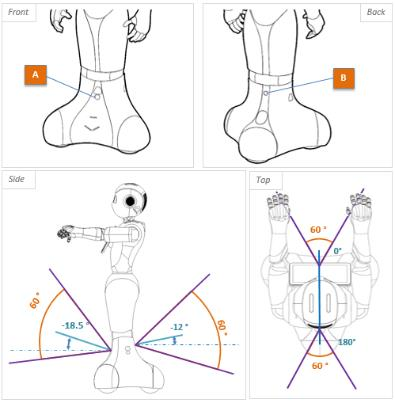
\includegraphics[width=\linewidth]{Figures/Pepper_Robot/sonars.jpg}
  \caption{Sonars}
  \label{fig:sonars}
\end{subfigure}%
\begin{subfigure}{.5\textwidth}
  \centering
  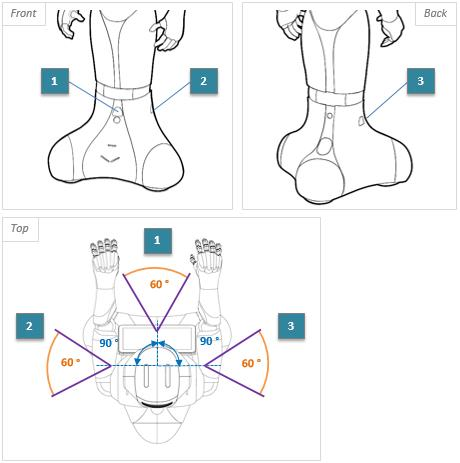
\includegraphics[width=\linewidth]{Figures/Pepper_Robot/lasers.jpg}
  \caption{Lasers}
  \label{fig:lasers}
\end{subfigure}
\caption{Positioning and field of vision of Pepper's sonars and lasers}
\label{fig:sonars_lasers}
\end{figure}

\begin{figure}[H]
\centering
\begin{subfigure}{.5\textwidth}
  \centering
  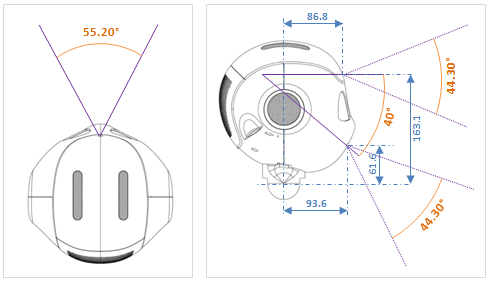
\includegraphics[width=\linewidth]{Figures/Pepper_Robot/2d_camera.png}
  \caption{2D Camera}
  \label{fig:2d_camera}
\end{subfigure}%
\begin{subfigure}{.5\textwidth}
  \centering
  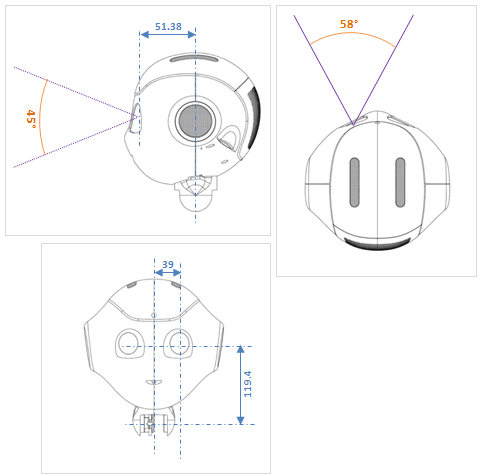
\includegraphics[width=\linewidth]{Figures/Pepper_Robot/3d_camera.png}
  \caption{3D Camera}
  \label{fig:3d_camera}
\end{subfigure}
\caption{Positioning and field of vision of Pepper's cameras}
\label{fig:cameras}
\end{figure}

\paragraph{} As for actuators, Pepper is equipped of omnidirectional wheels that allow it to turn in place and not be forced to face the direction it is translating toward. Two motors allow it to fold its body a little, just above the base and at the hips, but not enough for it to be able to touch the ground with its arms. Two motors allow the head to move forward/backward and turn left or right (but not for a full turn). Finally, it has two articulated arms including fingers, that are mainly meant for interactions with humans, but not for lifting large or heavy obstacles.

\paragraph{} All these characteristics are important, because they condition the way we can implement a navigation algorithm.

\subsection{On experimentation repeatability with ROS and Pepper}

\paragraph{} We mentioned at the beginning of our work that the \groupname \, uses ROS \footnote{ROS, the Robot Operating System, website: \url{http://www.ros.org/}} to program Pepper. ROS is a robotics middleware, and, in fact, not an operating system. It provides a high-level abstraction of hardware while still allowing for low-level device control, task distribution over a network capabilities, and most importantly, a message-passing system between processes, that allows a great diversity of programs written in many different languages to still be able to talk to one another. It also brings a package management system, that is coupled with the packaging system of the GNU/Linux distribution Ubuntu \footnote{Official website: https://www.ubuntu.com/}, allowing for plug-and-play capabilities for new software components.

\paragraph{} However, the versatile nature of ROS makes it very difficult to reproduce experiments \parencite{white_ros_2017}.

% TODO Add text here about Dockerfile, why use it, and what my variation with Pepper brings. Propose a modification on ROS wiki article for Pepper that links to my Doccker file? Keywords: Portable Linux ROS Workspace for Pepper with Docker.

\subsection{Experiment protocol}

% TODO Add text here about manipulation experiments done with Pepper and figures taken with Cylia and Lelio

\subsection{Results}

% Show photos of manipulations and conclude that the robot needs to be at the center of the obstacle in order to manipulate it properly.

\section{Simulation in a ROS-Standards compatible simulator}

\subsection{Simulator presentation}

% TODO Discuss why we could not just implement using ROS navigation stack

% TODO Discuss structure of the code and the viz in rviz

\subsection{Simulation results}

\paragraph{} At the time of the writing of this report, we were only able to implement the algorithm and the necessary simulation code for the base solution presented in section \ref{discussion_hypotheses_section}, but not the three propositions that build upon it. This still allowed us to validate all comments and improvements made in Chapter \ref{Chapter3} and in the first section of Chapter \ref{Chapter4}. Below are a few figures () showing a test case in a corridor with two obstacles.

% TODO take screenshots showing the simulator at work and put these here.
